\documentclass[runningheads]{llncs}
\usepackage[latin9]{inputenc}
\usepackage{url}
\usepackage{amsmath}
\usepackage{graphicx}
\usepackage[unicode=true,
 bookmarks=false,
 breaklinks=false,pdfborder={0 0 1},backref=section,colorlinks=false]
 {hyperref}

\makeatletter
%%%%%%%%%%%%%%%%%%%%%%%%%%%%%% User specified LaTeX commands.
% This is samplepaper.tex, a sample chapter demonstrating the
% LLNCS macro package for Springer Computer Science proceedings;
% Version 2.20 of 2017/10/04
%
% Used for displaying a sample figure. If possible, figure files should
% be included in EPS format.
%
% If you use the hyperref package, please uncomment the following line
% to display URLs in blue roman font according to Springer's eBook style:
% \renewcommand\UrlFont{\color{blue}\rmfamily}









\usepackage{listings}
\renewcommand{\lstlistingname}{Listing}



\usepackage{listings}
\renewcommand{\lstlistingname}{Listing}





\usepackage{listings}
\renewcommand{\lstlistingname}{Listing}



\makeatother

\usepackage{listings}
\renewcommand{\lstlistingname}{Listing}

\begin{document}
\title{Standardized crypto-loans on\\ the Cardano blockchain}%\thanks{Supported by Cardano Foundation.}}


\author{Dmytro Kondratiuk\inst{1}\orcidID{XXXX} \and
				Pablo {Lamela Seijas}\inst{1}\orcidID{0000-0002-1730-1219} \and
                Simon Thompson\inst{1,2}\orcidID{0000-0002-2350-301X}}

\authorrunning{D. Kondratiuk, et al.}

\institute{IOHK, Hong Kong,
\email{dmytro.kondratiuk@iohk.io, pablo.lamela@iohk.io, simon.thompson@iohk.io}  \and
School of Computing, University of Kent, UK,
\email{s.j.thompson@kent.ac.uk}}



%
\maketitle              % typeset the header of the contribution
%
\begin{abstract}
Crypto-loans are unique and innovative financial instruments that
allow trustless P2P lending, which could provide a safe and convenient
source of liquidity for cryptocurrency holders. In this article, we
explore a smart-contract framework for building standardized crypto-loans
with Marlowe DSL and Algorithmic Contract Types Unified Standards
at its core.

\keywords{Cardano \and ACTUS \and blockchain \and finance \and Marlowe \and Haskell} 
\end{abstract}


\section{Introduction}

List of contributions:
\begin{itemize}
\item \textquotedblleft Marlowe Labs\textquotedblright{} editor on Playground
(Dmytro) 
\item R Shiny cashflow visualiser for ACTUS (Dmytro) 
\item ACTUS Utility functions (Dmytro, Quanterall) 
\item executable ACTUS spec for PAM (Dmytro, Alex) 
\item executable ACTUS spec for LAM (Wyo Hackathon) 
\item Library for generating ACTUS contracts (Dmytro) 
\item ACTUS-like examples on Playground (Dmytro, Alex, Pablo) 
\item Marlowe DSL enhancements for Actus: Cond, Mul (Dmytro) (draft) 
\item ACTUS spec generator for Agda (Dmytro) 
\item Auto-refund static analysis (Pablo) (partial: only QC) 
\item Verification with QC + SMT (Dmytro) 
\end{itemize}

\section{Background}

A loan is a form of debt incurred by an individual or other entity.
The lender advances a sum of money to the borrower. In return, the
borrower agrees to a certain set of terms including any finance charges,
interest, repayment date, and other conditions \cite{loan}.

Cryptocurrency-backed loans must have collaterals as there is no trust
between party and counterparty. While loan is usually settled in a
stable-coin currency (e.g. USDT/USDC), the typical collateral is denominated
in a cryptocurrency (e.g. BTC). The purpose of this loan is to give
the borrower access to the fiat value of their crypto-funds without
actually selling them for fiat. Borrower pays interest In exchange
for provided liquidity.

Every loan has a positive net payoff (return minus investment) that
is either rendered as a one-time payment (see ZCB) or as a scheduled
payment of the interest. The rate of interest could be fixed throughout
the lifetime of a contract - for example zero-risk bonds have an fixed
interest proportional to inflation rate.

However, in a generic case - the interest rate is variable and depends
on an external factor agreed in advance, while the interest is periodically
updated by observing the state of that factor. Such loans usually
represent an investment in a particular venture or the industry. As
a somewhat fictional example, one could imagine a cryptocurrency miner
who decided to scale their crypto-farm: the loan (in USD) with variable
interest that directly depends on cryptocurrency prices would be more
attractive for a miner because it would directly correlate with miner's
profits. For example, if the price of the cryptocurrency goes down
in a particular month - miners would have to pay lower interest -
one always pays ``fixed share'' of the profits. In a more traditional
setup - the canonical example would be a power plant taking a loan
with interest depending on electricity prices. In both cases, either
cryptocurrency or electricity prices become a driver for the interest
rate.

Although, one can't just take the bare price of the asset and turn
it into a rate. In order to make ``units of measurement'' compatible
- adjustments should be made. Fluctuations of the interest rate driver
are embedded as:

\noindent 
\begin{equation}
\Delta_{r}=capfloor(driver*multiplier+spread-interestRate_{t-1})
\end{equation}

\noindent 
\begin{equation}
interestRate_{t+1}=capfloor(interestRate_{t-1}+\Delta_{r}),
\end{equation}

Where capfloor is a function that limits the range of fluctuation
(thus limiting lender's risk exposure):

\noindent 
\begin{equation}
capfloor(x)=max(min(x,floor),cap)
\end{equation}

Here, the spread parameter loosely represents the difference between
the average prime rate that the lender expects (benchmark yield) and
the rate imposed by the driver - the higher the spread, the higher
the resulting interest rate is. Multiplier effectively rescales the
interest rate plot in order to represent the difference between units
of measurement: how much percentage points you would get for a usd-to-kilowatt
and so on.

In the context of ACTUS and other event-based frameworks, there is
one more factor influencing interest rates thrrough scaling:

\noindent 
\begin{equation}
interestPayment=interestScalingFactor*interstRate*notional
\end{equation}

This scaling is dynamic and loosely adjusts for variance (volatility)
of the asset that the interest rate driver represents.

\paragraph*{Interest accrual and capitalisation. }

Counterparty might decide to reinvest profit received as interest
from the same loan. In the simplest case, this renders as compound
interest. This can be modeled through interest accrual and capitalisation,
for instance contracts from the ACTUS specification accrue interest
between interest payments and can transfer interest to a notional
during interest capitalisation event (IPCL).

Overall, variable interest rates introduce a certain risk for a lender,
thus they are subject to hedging. While any instrument that depends
on the same risk factor (interest rate driver) would suffice - the
most popular way to hedge a variable interest rate loan is interest
rate swap. This instrument allows two (or more) parties to exchange
their incomes - one from fixed interest rate loans, the other one
- from variable interest

\paragraph*{Counterparty risk.}

Trustless setups, especially ones in the cryptocurrency world (e.g.
decentralised smart-contracts and exchanges) require zero trust between
party and counterparty involved in a contract. In case of a loan,
this literally means that counterparty has zero-obligation to pay
the money back, thus rendering the loan useless for a party. Such
risks are usually addressed by introducing collaterals: 
\begin{enumerate}
\item Alice would like to borrow 1000 USD 
\item She has Bitcoin assets cost around 1500 USD, which she intends to
hold throughout a year, so Alice has high confidence in the market
(she expects prices to double or triple) 
\item Bob would like to lend 1000 USD and get an interest higher than traditional
interest rate offered by banks (let's say 15\% instead of 10\%). He
is either bearish or neutral towards Bitcoin. 
\item Alice transfers her BTC as collateral to a contract, and Bob transfers
his USD to Alice 
\item If Alice pays interest and notional on time (and Btc-price doesn't
render collateral worthless) - she can get her collateral back, otherwise
the loan gets liquidated and collateral is transferred to Bob. 
\end{enumerate}

\section{Modeling financial contracts}

\subsection{Marlowe }

Marlowe is a high-level, domain-specific language (DSL) for writing
financial contracts on blockchain\cite{marlowe}. Marlowe is defined
by an executable semantics in Haskell, and has been implemented on
the UTxO-based Cardano blockchain.

The main advantage of using Marlowe to carry ACTUS logic is enhanced
security that static analysis provides. SMT-solvers gain increasing
popularity as an alternative to fuzzing when it comes to testing software
for vulnerabilities\cite{smt}. Smart contracts generated from ACTUS
specification are quite complicated, so manually testing every possible
execution path for every possible combination of contract terms is
not feasible. Static analysis, in turn, can reduce the amount of ``dumb''
mistakes that could cost millions to the users by ensuring obvious
properties of a contract. It is not a panacea, however, unlike with
fuzzing, if SA says that certain property holds - it does it with
100\% assurance.

\subsection{ACTUS}

ACTUS defines the logic embedded in legal agreements that eventually
turn the contract terms into actual cash flows, or more generally
business events \cite{actus}. Most of its basic contract types represent
different variations of lending contracts.

ACTUS relies on a state machine formalism in order to describe the
behaviour of a given contract. Every payoff (transfer of funds in
or out of a contract) can be inferred for any given state. Every state
can be inferred from previous events and observed risk factors:

\noindent 
\begin{equation}
payoff_{i}=POF(state_{i})
\end{equation}

\noindent 
\begin{equation}
path=STF_{1}(ct,ev_{1})\circ STF_{2}(ct,ev_{2}).\circ\ldots\circ STF_{i}(ct,ev_{n})
\end{equation}

\noindent 
\begin{equation}
state_{i}=path(INIT(ct)),
\end{equation}

where $ct$ is contract terms, $INIT$ returns initial state, $sched$
returns scheduled events, $STF$ takes ${contractterms,event,state}$
and returns next state, $POF$ returns payoff.

\subsection{Necessity for Oracles}

In order to support variable interest rates and scaling, ACTUS requires
a smart contract to be able to observe the value of a given risk factor
(such as interest rate) at a particular point in time t:

\noindent 
\begin{equation}
riskfactor_{i}{}_{t}=O_{rf}(i,t)
\end{equation}

This is due to the risk factor's state not being known at instantiation
time. In the case of Cardano blockchain, these values are usually
provided through an ``Oracle'' mechanism\cite{oracles}. Oracle
could be a trusted party providing necessary data or network of parties
under consensus {[}find a quote{]}. From Marlowe DSL perspective,
the exact mechanism that provides external data is less important,
as Marlowe abstracts over IO by requiring particular type of input
(``Choice'') protected with a cryptographic signature (Choice owner).
As a result, the event of receiving data from Oracle is treated the
same as receiving integer numbers from user input in other languages

\section{Building executable specification of ACTUS}

\subsection{Mimicking the specification with Haskell code}

The ACTUS standard is specified in terms of scheduling, payoff and
state transition functions that are polymorphic on event and contract
type. The specification also follows quite specific naming conventions
that are incompatible with Haskell's conventions. The executable specification
follows original ACTUS conventions as close as possible in order to
ease code base maintenance when faced with updates of original ACTUS
spec (link to github).

Using Haskell itself as a DSL for explicitly encoding formulas without
using advanced language idioms also simplifies code generation, but
in case of ACTUS comes at a cost reduced type-safety, handling nullable
values explicitly introduces risk of exceptions. However this risk
is addressed using QuickCheck generators.

\subsection{Utilizing polymorphism to abstract over basic operations}

In order to keep our executable specification independent of the carrier
(whether its smart-contract engine, proof assistant, analytical framework
or even machine learning model) - we abstract over underlying representations
of state variables and arithmetic operations:

\begin{verbatim}
-- Definitions/ContractState.hs 
data ContractStatePoly a b = ContractStatePoly  
{  
tmd     :: b  
, nt    :: a  
, ipnr  :: a  
, ipac  :: a  
, feac  :: a  
, fac   :: a  
, nsc   :: a  
, isc   :: a  
, prf   :: ContractStatus  
, sd    :: b  
, prnxt :: a  
, ipcb  :: a  
} deriving (Show) 

-- Ops.hs
class ActusOps a where    
   _min :: a -> a -> a
   _max :: a -> a -> a
   _zero :: a
   _one :: a

class ActusNum a where
   (+) :: a -> a -> a
   (-) :: a -> a -> a
   (*) :: a -> a -> a
   (/) :: a -> a -> a

class YearFractionOps a b where
   _y :: DCC -> a -> a -> a -> b   

class DateOps a b where
   _lt :: a -> a -> b --returns pseudo-boolean   

class RoleSignOps a where
   _r :: ContractRole -> a
\end{verbatim}

Thus, every formula in the executable spec could either be instantiated
to: 
\begin{itemize}
\item formula on some ``atomic'' type (like Double, Day) - could be used
to directly compute cash-flows for analytical purposes or precompute
payoffs for smart contracts that don't depend on oracles 
\item formula representing piece of AST (Marlowe Value, Observation) - could
be used to generate smart contracts that depend on oracles or to generate
code in another language (like Agda) 
\end{itemize}
This approach of abstracting formulas has a limitation of not allowing
conditionals to be expressed in an abstract way (There is no ActusIf
typeclass) - luckily most of conditional expressions in ACTUS specification
don't depend on variable state of a contract - they depend on ContractTerms
that are known in advance during contract generation. This allows
us to dispatch appropriate formulas during generation rather than
execution.

The only exception to this are rare situations where we need to compare
2 state variables and either choose formula1 or 0 depending on comparison
result:

\begin{equation}
formula(st)=\begin{cases}
formula'(st) & var1(st)<var2(st)\\
0 & otherwise
\end{cases}
\end{equation}

We rely on pseudo-boolean ``less than'' function in order to address
that:

\noindent 
\begin{equation}
formula(st)=pseudoLt(var1(s1),var2(st)))*formula'
\end{equation}

\noindent 
\begin{equation}
pseudoLt(a,b)=Cond(a>b,1,0)
\end{equation}


\subsection{Contract terms representation and explicit applicability}

In order to simplify serialisation/deserialisation of contract terms
across Actus related services maintained by Cardano - we rely on ``superposed''
representation of contract terms - all ACTUS contract types are represented
with the same type. While such representation allows both encoder
and decoder to express any ACTUS contract terms, it also allows for
invalid combinations of terms (for example PRNXT cannot be applied
to PAM-contract), which means contracts require specific validation
that is implemented by means of applicability function:

\noindent 
\begin{equation}
Applicability:ContractTerms\mapsto Bool
\end{equation}

ACTUS defines a family of applicability functions polymorphic on contract
type (TODO link to ACTUS applicability):

\noindent 
\begin{equation}
Applicability:ContractType\times ContractTerm\mapsto ApplicabilityType,
\end{equation}

where applicability could be: none, always, nullable, multiple

In order to build superposed contract terms type for such function,
we have to resolve conflicting applicability for contract terms merged
using the following resolution rules:

\noindent 
\begin{equation}
weaken(a_{1},a_{2})=\begin{cases}
nullable & a_{1}=none\wedge a_{2}=always\\
nullable & a_{1}=always\wedge a_{2}=none\\
a_{1} & priority(a_{1})>priority(a_{2})\\
a_{2} & otherwise
\end{cases}
\end{equation}

\noindent 
\begin{equation}
priority(x)=\begin{cases}
0 & x=always\\
1 & x=none\\
2 & x=nullable\\
3 & x=multiple
\end{cases}
\end{equation}

Where $a_{1}$ - is applicability of a given term of first contract
type to be merged $a_{2}$ - is applicability of a given term of second
contract type to be merged

\section{Generating Marlowe contracts from standardised ACTUS contract terms}

\subsection{Overall architecture }

\begin{figure}
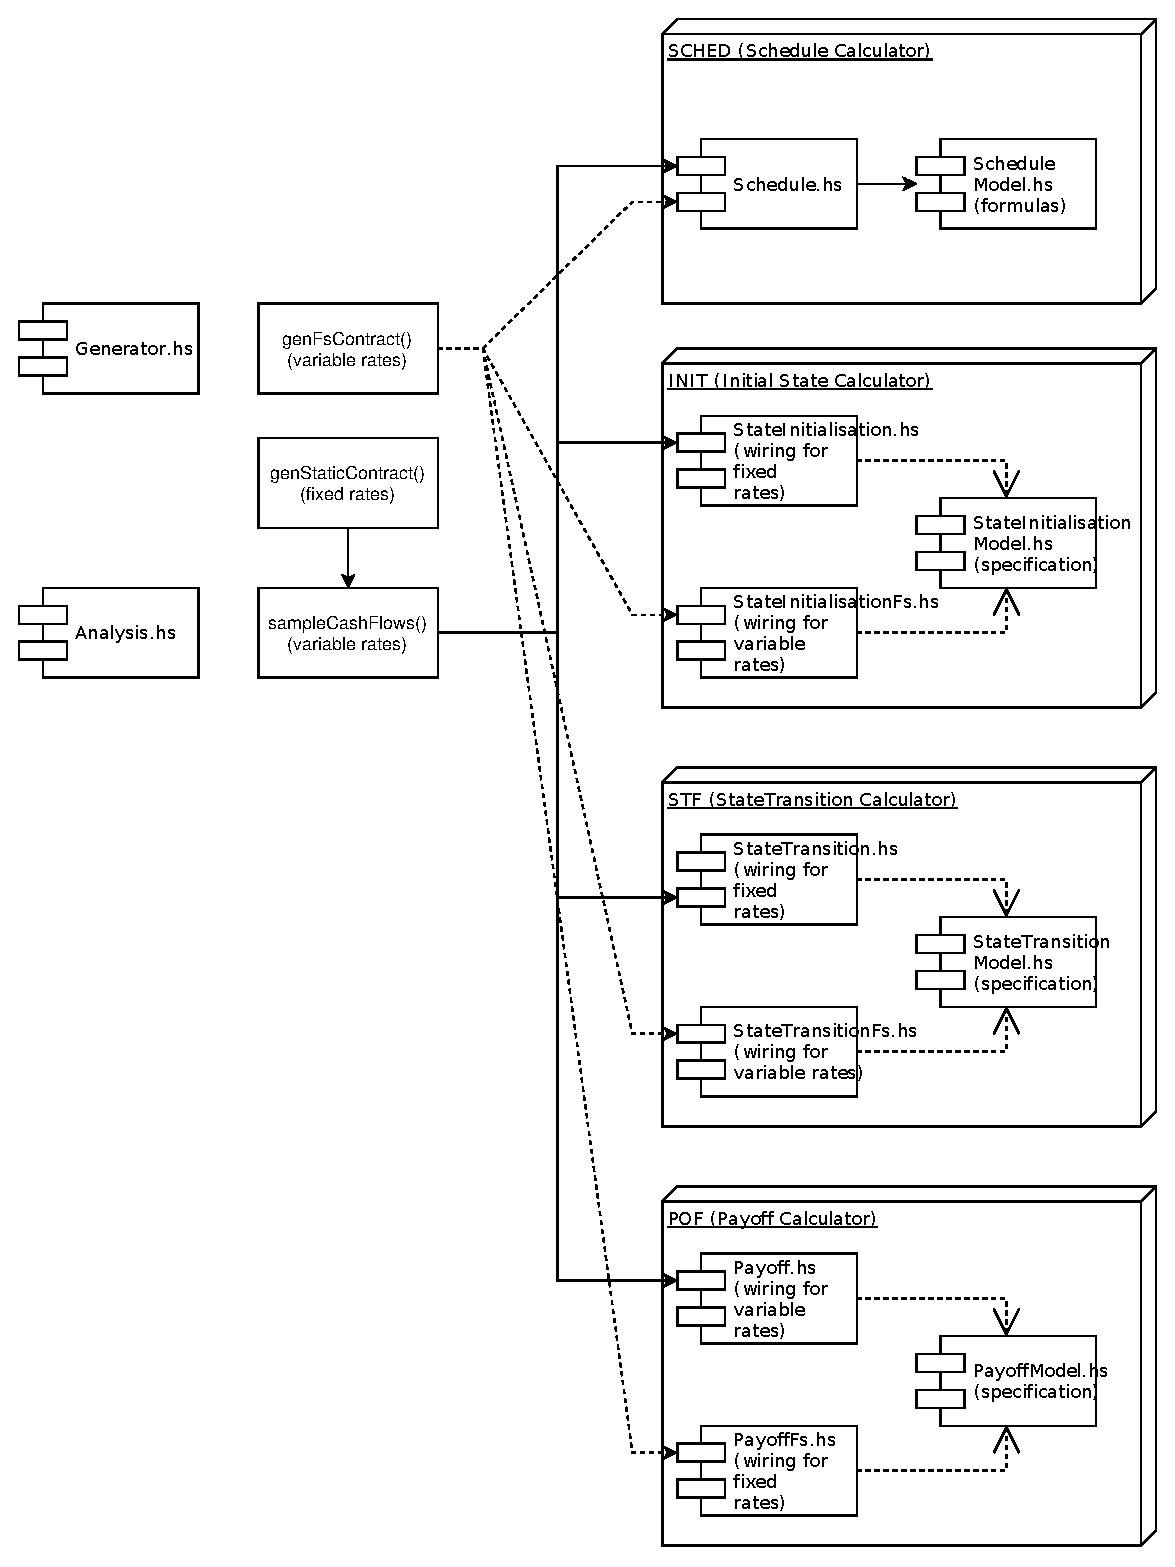
\includegraphics[width=1\textwidth]{images/modules} \caption{Modules responsible for contract generation.}
\label{fig1} 
\end{figure}

Generated contract is essentially a continuation chain of smaller
contracts:

\noindent 
\begin{equation}
chainlink(t)=receiveData(t)\circ calculatePayoff(t)\circ processPayoff(t)
\end{equation}

\noindent 
\begin{equation}
contract(ct)=collaterals(ct)\circ INIT(ct)\circ\prod_{t\in SCHED(ct)}chainlink(t)
\end{equation}

where $receiveData$ - is asking an oracle for Marlowe Choice if needed,
$calculatePayoff$ - calculates payoff formula. For fixed-rate contracts
this is optimised into a precalculated constant. $processPayoff$
- awaits Deposit of payoff amount from a party: if deposit is transferred
it redirects the funds to a counterparty - otherwise it transfers
the collateral to a counterparty and closes the contract. The chain
is generated from the fixed (known in advance) schedule of events
using $SCHED()$function from ACTUS.

\begin{figure}
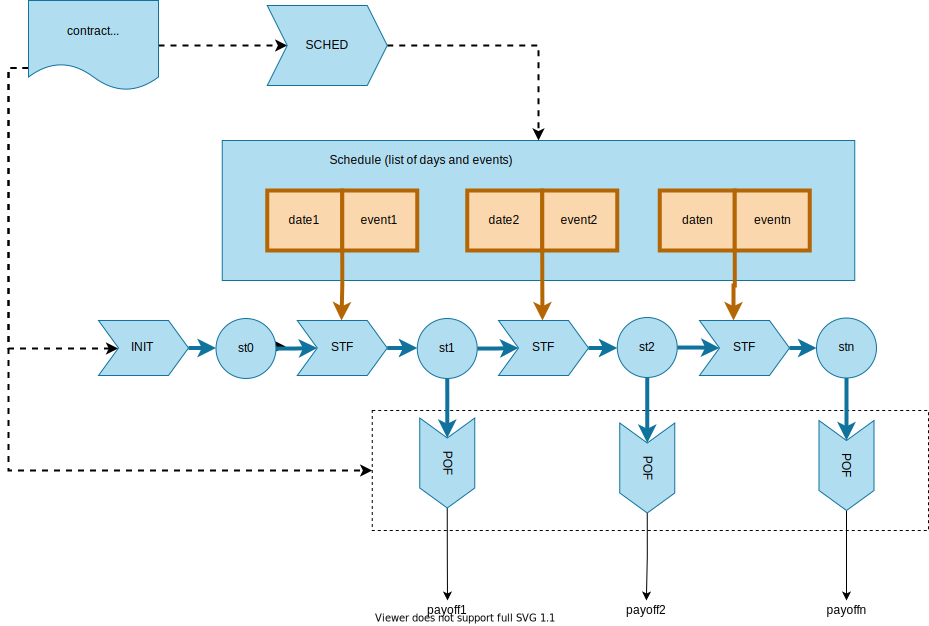
\includegraphics[width=1\textwidth]{images/flowchart} \caption{Chain of sub-contracts representing ACTUS logic}
\label{fig2} 
\end{figure}


\subsection{Avoiding exponential growth }

Marlowe doesn't allow functions and recursion. Naive usage of If operator
in Marlowe could lead to exponential growth of a contract, for example:

\begin{verbatim}
if condition 
	then 
		perform_something1()
		continue() 
	else 
		perform_something2 
		continue()
\end{verbatim}

would inline contents of $continue()$ twice and given that ACTUS
contracts are essentially generated using continuation as an accumulator
- this would lead to exponential explosion of the size of any actus
contract that has conditionals in their state transition logic.

Example of such logic would be cap/floor limitations on interest rate:

\noindent 
\begin{equation}
adjusted=max(min(original,floor),cap)
\end{equation}

We addressed this issue by introducing ``Cond'' construct in order
to represent ``if'' expressions. So instead of using the ``If''
contract to decide the value of some variable - we use conditional
assignment instead as ``Cond'' is essentially just a pure function
that returns value depending on condition in contrast to the ``If''
contract that performs action instead of returning value. The name
is borrowed from a similar function in Lisp.

\subsection{Limitations due to termination }

Marlowe doesn't allow perpetual contracts even if their recursion
is productive (example: perpetual swap) - thus we can't support certain
contract types from ACTUS specification, namely the ones that don't
have a defined maturity date (like UMP). In a long-term perspective
- there is a possible workaround: contracts with no maturity date
could be represented as actors with finite amounts of state transitions.
We prototyped this approach in a separate branch, however it does
seem more prone to errors comparing to rendering predefined schedules
and more importantly it greatly affects static analysis as the amount
of ``reduction steps'' grows from $N_{scheduled}=count(event)$
to $N_{stateTransitions}=\frac{max(date(event))-min(date(event))}{precision}$. 

\subsection{Fixed-point precision }

Marlowe only supports Integers, while ACTUS is expressed in terms
of real numbers. In order to model a real number in such a setup -
we rely on fixed point precision. The algebra looks like this: 
\begin{verbatim}
(+)   = AddValue
(-)   = SubValue
a * b = Scale (1 % marloweFixedPoint) $ MulValue a b
\end{verbatim}


\subsection{Representing Actus state in a Marlowe contract}

Unfortunately, Marlowe DSL doesn't support any notion of records,
the variables can only be of type ``Integer''. Thus, in order to
map contract state (ContractStatePoly) we first pack a set of Marlowe
variables (Value Observation) representing previous $t-1$ state into
ContractStatePoly, then we apply polymorphic state transition, and
finally unpack ContractState poly into a set of Marlowe variables
into $t+1$ state:

\noindent 
\begin{equation}
st_{t+1}=unpack(stateTransition(pack(st_{t-1}))),
\end{equation}

,where pack is a chain of ``UseValue'' and unpack is a chain of
``Let''

\paragraph{Representing state transitions in Marlowe (unfolding)}

Marlowe doesn't support mutable variables, so we have to represent
state at t ($st_{t}$) literally through naming convention:

\begin{verbatim}
variableName(name, t) = 
	concat(name, '_', t) 
generateAccessor(name, t) = 
	UseValue variableName(name, t) 
generateSetter(name, t, formula) = 
	Let variableName(name, t) formula 
\end{verbatim}


\subsection{ActusLabs}

\begin{figure} 
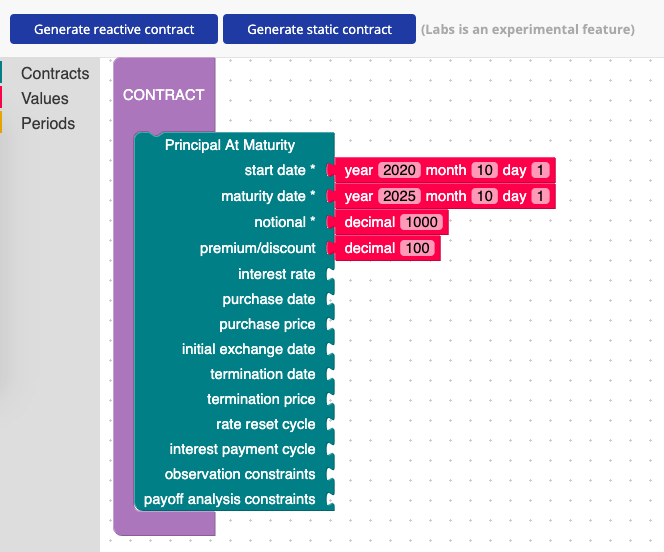
\includegraphics[width=0.8\textwidth]{images/labs.png}
\caption{Actus Labs - online tool for generating Actus contracts for Marlowe.} 
\label{fig3} 
\end{figure} 

In order to demonstrate and test the capabilities of Actus generators,
a visual online Blockly-based tool was developed for Marlowe Playground.
The Actus Labs tool allows users to construct contract terms visually,
generate a corresponding Marlowe contract and try it out in a simulated
environment.

\section{Tokenization}

Every participant of an ACTUS contract is described by a Role which
is in its turn represented through a special unique non-fungible token.
This makes every Marlowe contract a tradable security, allowing a
participant to sell its ``share'' in a contract by selling a corresponding
role token.

Role tokens can potentially allow more complex manipulation over shares,
especially when share represents an incoming cash flow: participants
only send funds to a party represented by a given token. Such a token
would represent a positive cashflow which in turn could not just become
tradable but would also allow to derive tokens only representing fractions
of a particular cash flow in a contract.

Moreover, it turns Actus-loans into derivatives, for example contracts
like Interest Rate Swap (and Swaps in general) could be approximated
by an Atomic Swap of tokens representing incoming cash flows from
lending.

For example, if Alice has fixed income from a loan (or some other
investment) and Bob has comparable but variable (fluctuating) income
- Bob can hedge by swapping cash flows with Alice. If Alice's income
is locked with token1 and Bob's income is locked with token2 - then
atomic swap of those tokens is equivalent to a swap of cash flows.

\section{Verification and testing}

\subsection{QuickCheck for cross-testing}

In order to test the equivalence between Executable Haskell implementation
of ACTUS for smart-contracts and original Java implementation for
analytics - a simple property test was introduced:

\noindent 
\begin{equation}
\forall ct\forall rf.getCashFlows("haskell",ct,rf)\equiv getCashFlows("java",ct,rf)
\end{equation}

Where $ct$ represnts contract terms, $rf$ is risk factor model and
$getCashFlows()$ returns a set of $(date,payoff)$ tuples.

\subsection{QuickCheck for verification}

QuickCheck\cite{qc} contract terms generators also allow to ensure
arbitrary properties of a Marlowe contract. This could be enhanced
with Marlowe's static analysis feature by utilising Assert operator:

\begin{verbatim}
ContractTerms := sample(qcgenerator) 
Contract := generateMarloweContract(ContractTerms) 
ContractWithAssert := appendAssertion(Contract, assertion) 
runStaticAnalysis(ContractWithAssert)
\end{verbatim}

While it doesn't cover all possible contracts it could guarantee that
property holds for a statistically significant fraction of a contract.
Using Static Analysis to check a particular contract instead of randomly
sampling allows: 
\begin{itemize}
\item more balanced sampling: Space of contract terms depends linearly on
the coverage, e.g. if we cover 10\% of all possible contract terms
- we'll cover 10\% of all contracts. Different contracts have different
amount of risk factors thus different search space, for instance a
contract with 3 risk factors (e.g. 3 observations of an interest rate)
would span over n\textasciicircum 3 while a contract with 10 risk
factors would span over n\textasciicircum 10. Meanwhile, space of
all risk factors in all contracts doesn't linearly depend on the coverage. 
\item dependency tracking: SMT-solver would likely be more aware of execution
paths leading to failure of a test, which could significantly reduce
search space 
\item completeness: If not timed out, SMT-solver is decidable while sampling
is semi-decidable. 
\end{itemize}

\subsection{Securing collateral logic with auto-refund warnings}

By design, the Marlowe interpreter always refunds assets held in a
contract when it terminates. This is done in order to ensure that
no funds are lost forever. The funds are returned to whoever's internal
account actually holds them.

However, this presents as a problem in certain cases where ownership
of the funds could not be automatically determined. For example if
Alice puts collateral in a crypto-loan contract - she would formally
maintain ownership, which means she would get automatically refunded
when Close contract is reached.

This implicit refund is easy to overlook by smart-contract developers
as plain Close is often used as a default action in case of unexpected
behaviour like timeouts(especially Choice timeout). This can easily
lead to multi-million dollar mistakes if malicious Alice decides to
exploit an auto-refund feature in order to get her collateral without
paying back. Here's the example of simple attack vector: 
\begin{enumerate}
\item Alice creates a contract where Deposit timeout would lead to Close 
\item Bob doesn't know or test the timeout path. Even if Bob is a programmer
- he might not be aware that Closing contract would cause collateral
refund 
\item Alice puts collateral and gets notional from Bob 
\item Alice doesn't pay for a loan (Deposit timeout) 
\item Alice gets her collateral back 
\item Bob loses notional 
\end{enumerate}
In order to prevent this from happening, an additional ''Auto-Refund''
security check was introduced as part of Static Analysis tooling which
notifies users about all ``Close'' constructs that can lead to automatic
refunds and encourages users to write explicit logic for edge cases.

\section{Comparison with existing smart-contracts approaches }

Unlike current popular DeFi lending approaches - Marlowe ACTUS-based
implementation tends to rely on trade-matching instead of pooling.
While asset pooling is proven to be superior to order-book based approaches
when it comes to automated market makers, using it for lending has
been shown to be more susceptible to attacks\cite{flash-loan}.

Moving trade matching off-chain also improves scalability of the protocol
- every loan is a separate contract, thus there is no global state.

Actus provides additional benefit of being regulatory friendly, ACTUS
foundation provides a set of tools allowing Monte-Carlo simulations
of ACTUS contracts.

\section{Conclusion}

Marlowe language was explicitly designed as a set of building blocks
for financial contracts that could be combined by anyone familiar
with basic programming. Marlowe ACTUS generators improve on that by
providing a way to automatically combine blocks based on standardized
requirements specified by the user.

On top of that, Marlowe ACTUS provides a toolkit for cross-testing
with original ACTUS spec, a framework for adding new contract types,
cash-flow visualisations and verification tooling.

%
% ---- Bibliography ----
%
% BibTeX users should specify bibliography style 'splncs04'.
% References will then be sorted and formatted in the correct style.
%
\bibliographystyle{splncs04}
\bibliography{article}
%

\end{document}
